\documentclass[11pt,letterpaper,openany]{book}

% Essential packages
\usepackage[T1]{fontenc}
\usepackage[utf8]{inputenc}
\usepackage{lmodern}
\usepackage[margin=1in]{geometry}
\usepackage{microtype}
\usepackage{graphicx}
\usepackage{float}
\usepackage{xcolor}
\usepackage{titlesec}
\usepackage{tocloft}
\usepackage{fancyhdr}
\usepackage{hyperref}
\usepackage{bookmark}
%\usepackage{glossaries}
%\usepackage{imakeidx}
\usepackage{listings}
\usepackage{tcolorbox}
\usepackage{caption}
\usepackage{amsmath}
\usepackage[nameinlink]{cleveref}
\usepackage{booktabs}
\usepackage{etoc}
\usepackage{tikz}
\usetikzlibrary{arrows,shapes,positioning,shadows,trees}

% Color definitions based on brand palette
\definecolor{primarydark}{RGB}{0,43,86}  % Darkest blue
\definecolor{primary}{RGB}{65,146,206}  % Mid blue
\definecolor{primarylight}{RGB}{188,223,242}  % Lightest blue
\definecolor{secondarydark}{RGB}{29,143,143}  % Darkest teal
\definecolor{secondary}{RGB}{95,201,201}  % Mid teal
\definecolor{secondarylight}{RGB}{190,235,235}  % Lightest teal
\definecolor{accentdark}{RGB}{193,113,67}  % Darkest brown
\definecolor{accent}{RGB}{226,172,140}  % Mid brown
\definecolor{accentlight}{RGB}{242,219,205}  % Lightest brown
\definecolor{alertdark}{RGB}{205,65,65}  % Darkest red
\definecolor{alert}{RGB}{233,137,137}  % Mid red
\definecolor{alertlight}{RGB}{247,205,205}  % Lightest red

% Chapter and section styling
\titleformat{\chapter}[display]
{\normalfont\huge\bfseries\color{primarydark}}
{\chaptertitlename\ \thechapter}{20pt}{\Huge}
\titleformat{\section}
{\normalfont\Large\bfseries\color{primary}}
{\thesection}{1em}{}
\titleformat{\subsection}
{\normalfont\large\bfseries\color{primarydark}}
{\thesubsection}{1em}{}

% Table of contents styling
\renewcommand{\cftsecleader}{\cftdotfill{\cftdotsep}}
\renewcommand{\cftchapfont}{\color{primarydark}\bfseries}
\renewcommand{\cftsecfont}{\color{primary}}
\renewcommand{\cftsubsecfont}{\color{primarydark}}

% Header and footer styling
\pagestyle{fancy}
\fancyhf{}
\fancyhead[LE,RO]{\thepage}
\fancyhead[LO]{\nouppercase{\rightmark}}
\fancyhead[RE]{\nouppercase{\leftmark}}
\fancyfoot[C]{\textcolor{primary}{\rule{0.5\textwidth}{0.4pt}}}

% Hyperref setup
\hypersetup{
    colorlinks=true,
    linkcolor=primarydark,
    filecolor=accent,
    urlcolor=secondary,
    pdftitle={The IT Consultant's Automation Handbook},
    pdfauthor={Dele Tosh},
    pdfsubject={IT Consulting and Automation},
    pdfkeywords={BPA, RPA, business process automation, n8n, Budibase},
}

% Glossary setup
%\makeglossaries

% Index setup
%\makeindex

% Custom box styles
\newtcolorbox{warningbox}{
    colback=alertlight,
    colframe=alertdark,
    title=Warning,
    fonttitle=\bfseries
}

\newtcolorbox{importantbox}{
    colback=secondarylight,
    colframe=secondarydark,
    title=Important,
    fonttitle=\bfseries
}

% Listing style
\lstset{
    basicstyle=\ttfamily\small,
    breaklines=true,
    commentstyle=\color{accentdark},
    keywordstyle=\color{primarydark},
    stringstyle=\color{alertdark},
    numbers=left,
    numberstyle=\tiny\color{primary},
    numbersep=5pt,
    frame=single,
    framesep=5pt,
    rulecolor=\color{primary},
}

% Caption style
\captionsetup{
    font=small,
    labelfont={\bfseries\color{primarydark}},
    margin=10pt
}
% Detailed table of contents
\etocsettocstyle{\subsubsection*{Contents}}{}

\setlength{\headheight}{14pt}


% Add these new packages if not already included
\usepackage{afterpage}
\usepackage{wrapfig}

% For formatting the date
\usepackage[useregional]{datetime2}

% Custom command for formatting the date
\newcommand{\monthyeardate}{%
    \DTMenglishmonthname{\@dtm@month}, \@dtm@year
}


\begin{document}

    \frontmatter

    \begin{titlepage}
        \centering
        \vspace*{2cm}
        {\Huge\bfseries\color{primarydark} The IT Consultant's\\ Automation Handbook\par}
        \vspace{2cm}
        {\Large\itshape Dele Tosh\par}
        \vspace{1cm}
        {\large Founder \& Director, Protomated.com\par}
        \vfill
        {\large \currentmonthyear\par}
    \end{titlepage}

    \tableofcontents
%    \listoffigures
%    \listoftables

    \mainmatter

    \chapter*{Introduction: The New Era of IT Consulting}

If you're running a small IT consulting firm, you're likely all too familiar with the daily grind: drowning in manual tasks, struggling to meet client deadlines, and watching more tech-savvy competitors zoom past you. You know you need to innovate, but finding the time feels impossible. Sound familiar?

You're not alone. The IT consulting landscape is shifting rapidly, and small firms are feeling the pressure. But here's the good news: you're holding the key to not just surviving, but thriving in this new era.


\section{Why This Book, Why Now?}

The consulting world is undergoing a seismic shift. According to Deloitte's recent report, ``Unleashing value from digital transformation: Paths and pitfalls,'' the days of strategy-only consulting are numbered. Clients now demand execution, and technology is at the heart of it all.

Consider this: 30 years ago, classic strategy work made up 60-70\% of consulting engagements. Today? It's down to a mere 20\%. The message is clear: consultants who can't deliver tangible, tech-driven results will be left behind.

But here's where it gets exciting for small firms like yours. The report also highlights a crucial trend: the rise of specialist boutique firms. With the right tools and knowledge, you can deliver outcomes that rival the big players, at a fraction of the cost.

This is where automation comes in. It's not just a buzzword; it's your ticket to:
\begin{itemize}
    \item Boosting productivity by eliminating time-consuming manual tasks
    \item Consistently meeting (and exceeding) client deadlines
    \item Taking on more projects without burning out
    \item Positioning yourself as an innovation leader
    \item Finally achieving that elusive work-life balance
\end{itemize}


\section{What You'll Learn}

This book is your practical guide to leveraging no-code automation tools to revolutionize your IT consulting practice. We'll focus on three powerful platforms: n8n, nocodb, and budibase. By the time you finish this book, you'll know how to:

\begin{enumerate}
    \item Automate repetitive tasks to free up your time for high-value work
    \item Deliver unprecedented value to clients (and find new ways to monetize your automation skills)
    \item Scale your practice without working 80-hour weeks
    \item Integrate cutting-edge technologies like generative AI and cloud computing into your solutions
\end{enumerate}


\section{How to Use This Book}

Whether you're a complete newcomer to automation or you've dabbled a bit, this book is designed to meet you where you are. Each chapter builds on the last, providing a mix of theory, practical examples, and hands-on exercises.

We'll start with quick wins you can implement today, then progress to more advanced strategies. By the end, you'll have a comprehensive 90-day plan to transform your practice.

Don't just read passively. The real magic happens when you apply these concepts to your own business. So grab your laptop, roll up your sleeves, and get ready to join the ranks of innovative, future-proof IT consultants.

Ready to stop drowning in busywork and start leading the pack?

Let's dive in.
    \chapter{No-Code Tools Every IT Consultant Should Master}


\section{Introduction}

In today's fast-paced tech landscape, the ability to rapidly prototype and deploy solutions is invaluable. No-code platforms are revolutionizing how IT consultants work, allowing you to create powerful applications and automations without writing a single line of code. Let's dive into the top tools you need in your arsenal and explore real-world applications that can transform your consulting practice.


\section{Top 3 No-Code Platforms for IT Consulting}

\subsection{n8n (self-hostable)}

n8n is a powerful, flexible workflow automation tool that's perfect for IT consultants looking to build complex, customized solutions.

\textbf{Pros:}
\begin{itemize}
    \item Advanced capabilities for complex workflows
    \item Self-hostable for enhanced security and control
    \item Excellent for rapid prototyping and idea validation
    \item Can function as a low-code business ideas maker
    \item Ability to build entire backend software services
\end{itemize}

\textbf{Cons:}
\begin{itemize}
    \item Steeper learning curve compared to some alternatives
    \item GUI can become challenging to manage with very complex workflows
    \item Less polished UI compared to some competitors
\end{itemize}

\textbf{Real-World Use Case: Automated Incident Response System}

One of our clients, a medium-sized managed service provider, used n8n to create an automated incident response system. Here's how it works:

\begin{enumerate}
    \item The system monitors their ticketing system (Zendesk) for new high-priority tickets.
    \item When a critical ticket is created, n8n triggers a workflow that:
    \begin{itemize}
        \item Sends an alert to the appropriate team in Slack
        \item Creates a video call link in Zoom for immediate team collaboration
        \item Starts a timer to track response time
        \item Pulls relevant documentation from their knowledge base
        \item Updates the ticket with the collected information
    \end{itemize}
    \item If the ticket isn't addressed within 15 minutes, it escalates the alert to senior management.
\end{enumerate}

This automation reduced their average response time for critical incidents from 45 minutes to under 10 minutes, significantly improving their service level agreements (SLAs) and client satisfaction.

\subsection{NoCoDB (self-hostable)}

NoCoDB is an open-source Airtable alternative that provides a powerful, flexible database solution.

\textbf{Pros:}
\begin{itemize}
    \item Can import data from various sources, including Airtable
    \item Supports multiple database types (MySQL, Postgres, SQLite, SQL Server)
    \item Multilingual support
    \item Open-source and self-hostable
\end{itemize}

\textbf{Cons:}
\begin{itemize}
    \item Learning curve can be steep for non-technical users
    \item Lacks built-in cloud backup system
\end{itemize}

\textbf{Real-World Use Case: Centralized Client Management System}

A boutique IT consulting firm used NoCoDB to create a centralized client management system. They set up tables for:

\begin{itemize}
    \item Clients (with contact information, project history, and preferences)
    \item Projects (linked to clients, with timelines, budgets, and status updates)
    \item Resources (team members, equipment, and their availability)
    \item Invoices (linked to projects and clients, with payment status)
\end{itemize}

They then created views that allowed them to:

\begin{itemize}
    \item See all active projects and their status at a glance
    \item Track billable hours and project profitability
    \item Manage resource allocation across projects
    \item Generate custom reports for clients and internal stakeholders
\end{itemize}

This system replaced their previous combination of spreadsheets and a CRM, providing a more flexible and integrated solution that scaled with their business. They estimated it saved them 15-20 hours per week in administrative tasks.

\subsection{BudiBase (self-hostable)}

BudiBase is a low-code platform for creating web applications quickly and efficiently.

\textbf{Pros:}
\begin{itemize}
    \item Can connect to REST APIs
    \item Supports user role definition
    \item Open-source and self-hostable
    \item Features useful components like the repeater field
\end{itemize}

\textbf{Cons:}
\begin{itemize}
    \item Building complex UIs can be challenging
    \item Limited ability to use JavaScript for data manipulation in all components
    \item Less dynamic compared to some alternatives like Appsmith
\end{itemize}

\textbf{Real-World Use Case: Custom Client Portal}

An IT consultant specializing in data analytics used BudiBase to create a custom client portal for a large e-commerce client. The portal included:

\begin{itemize}
    \item A dashboard showing real-time sales data, inventory levels, and customer analytics
    \item A tool for generating custom reports based on user-selected parameters
    \item An interface for managing product listings across multiple platforms (Amazon, Shopify, eBay)
    \item A ticketing system for the client to request changes or report issues
\end{itemize}

The consultant connected BudiBase to the client's existing databases and APIs, creating a unified interface that pulled data from multiple sources. This portal replaced several disconnected tools the client was using, streamlining their operations and providing more actionable insights.

The consultant was able to deliver this solution in just three weeks, a fraction of the time it would have taken to develop a custom application from scratch. The client was so impressed with the result that they referred the consultant to two other businesses, leading to significant growth in the consultant's practice.


\section{Build Your First No-Code App in 30 Minutes}

Let's put theory into practice by building a client onboarding automation using n8n and NoCoDB. This practical example will demonstrate how quickly you can create valuable solutions for your consulting business.

\subsection{Setting Up Your Environment}

1. Ensure you have n8n and NoCoDB installed and running on your system.
2. Set up a Google Workspace account for integrations.

\subsection{Creating the NoCoDB Database}

Create a new table in NoCoDB with the following fields:
\begin{itemize}
    \item Client Name
    \item Company
    \item Email
    \item Phone
    \item Project Type
    \item Start Date
    \item Assigned Team Members
    \item Initial Meeting Date
    \item Document Status
    \item Project Folder Link
\end{itemize}

Now, let's create our n8n workflow:

1. \textbf{Trigger: New Form Submission}
Set up a Webhook node to receive new client data.

% TODO @screenshot: Webhook node configuration in n8n for receiving new client data

2. \textbf{Create NoCoDB Record}
Use the NoCoDB node to create a new record with the received data.

% TODO @screenshot: NoCoDB node configuration in n8n for creating a new record

3. \textbf{Create Google Drive Folder}
Utilize the Google Drive node to create a new folder for the client.

% TODO @screenshot: Google Drive node configuration in n8n for creating a new client folder

4. \textbf{Send Welcome Email}
Configure the Gmail node to send a personalized welcome email.

% TODO @screenshot: Gmail node configuration in n8n for sending a personalized welcome email

5. \textbf{Create Calendar Event}
Use the Google Calendar node to schedule the initial meeting.

% TODO @screenshot: Google Calendar node configuration in n8n for scheduling the initial meeting

6. \textbf{Update NoCoDB Record}
Finally, update the NoCoDB record with the folder link and meeting details.

% TODO @screenshot: Final NoCoDB update node configuration in n8n

\subsection{Testing and Activating Your Workflow}

Once you've connected all the nodes, it's time to test your workflow:

1. Use the n8n testing feature to simulate a new client submission.
2. Check each step of the workflow to ensure data is flowing correctly.
3. Verify that the NoCoDB database is updated, the Google Drive folder is created, the welcome email is sent, and the calendar event is scheduled.

% @illustrate: Complete workflow diagram showing all connected nodes in n8n
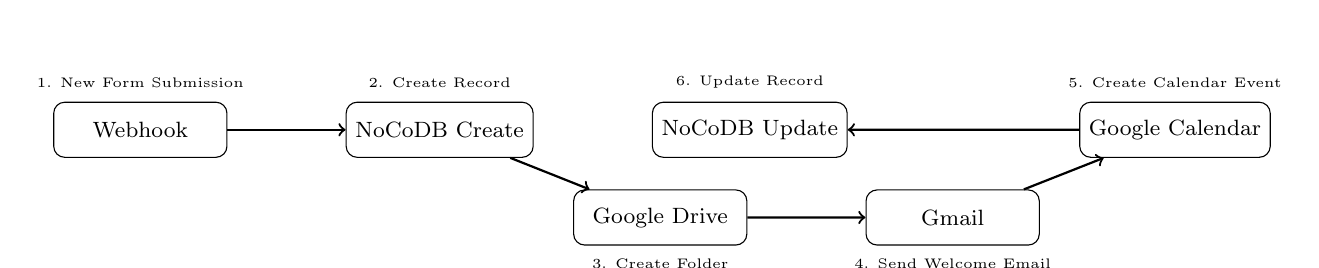
\begin{tikzpicture}
    [
    node distance = 0.8cm and 1.5cm,
    box/.style = {draw, rectangle, minimum width=2.2cm, minimum height=0.7cm, text centered, rounded corners, font=\footnotesize},
    arrow/.style = {->, thick},
    scale=0.85
    ]

% Nodes
    \node[box] (webhook) {Webhook};
    \node[box, right=of webhook] (nocodb1) {NoCoDB Create};
    \node[box, below right=0.4cm and 0.5cm of nocodb1] (gdrive) {Google Drive};
    \node[box, right=of gdrive] (gmail) {Gmail};
    \node[box, above right=0.4cm and 0.5cm of gmail] (gcal) {Google Calendar};
    \node[box, right=of nocodb1] (nocodb2) {NoCoDB Update};

% Arrows
    \draw[arrow] (webhook) -- (nocodb1);
    \draw[arrow] (nocodb1) -- (gdrive);
    \draw[arrow] (gdrive) -- (gmail);
    \draw[arrow] (gmail) -- (gcal);
    \draw[arrow] (gcal) -- (nocodb2);

% Labels
    \node[above=0.05cm of webhook, font=\tiny] {1. New Form Submission};
    \node[above=0.05cm of nocodb1, font=\tiny] {2. Create Record};
    \node[below=0.05cm of gdrive, font=\tiny] {3. Create Folder};
    \node[below=0.05cm of gmail, font=\tiny] {4. Send Welcome Email};
    \node[above=0.05cm of gcal, font=\tiny] {5. Create Calendar Event};
    \node[above=0.05cm of nocodb2, font=\tiny] {6. Update Record};

\end{tikzpicture}

Congratulations! You've just created a powerful client onboarding automation in under 30 minutes. This workflow will save you hours of manual work for each new client, allowing you to focus on delivering value rather than managing administrative tasks.


\section{Security and Compliance Considerations}

When working with no-code tools, especially in IT consulting where you're handling sensitive client data, security and compliance should be top priorities. Here are some key considerations:

1. \textbf{Data Privacy}: Ensure that your no-code platforms are compliant with relevant data protection regulations (e.g., GDPR, CCPA).

2. \textbf{Access Control}: Implement strict user access controls, especially when using self-hosted solutions.

3. \textbf{Data Encryption}: Use encryption for data at rest and in transit.

4. \textbf{Regular Audits}: Conduct regular security audits of your no-code setups.

5. \textbf{Backup and Recovery}: Implement robust backup solutions, especially for self-hosted platforms.

6. \textbf{Third-Party Integrations}: Carefully vet any third-party services you integrate with your no-code tools.

Remember, while no-code platforms can significantly speed up development, they don't absolve you of responsibility for the security and compliance of your solutions. Always approach these tools with a security-first mindset.


\section{Conclusion}

No-code tools like n8n, NoCoDB, and BudiBase are revolutionizing how IT consultants work. By mastering these platforms, you can deliver solutions faster, take on more complex projects, and provide greater value to your clients. The client onboarding automation we built and the real-world examples we explored are just the beginning – the possibilities are truly endless.

These tools allow you to:

\begin{itemize}
    \item Rapidly prototype and deploy solutions, reducing time-to-market
    \item Create custom, scalable applications without extensive coding knowledge
    \item Integrate disparate systems and data sources more easily
    \item Offer more competitive pricing by reducing development time
    \item Expand your service offerings to include areas previously out of reach
\end{itemize}

In the next chapter, we'll explore how to transform your core services using these no-code tools, opening up new revenue streams and enhancing your existing offerings.

\begin{importantbox}
    Remember, the key to success with no-code tools is to start small, experiment often, and continuously build on your successes. Each project you complete will expand your capabilities and open up new opportunities for your consulting practice.
\end{importantbox}

\textbf{Action Items:}
\begin{enumerate}
    \item Take the workflow we built in this chapter and customize it for your own business. What other steps could you add to make your client onboarding even more efficient?
    \item Choose one of the real-world use cases we discussed and brainstorm how you could implement a similar solution for one of your clients.
    \item Sign up for free accounts on n8n, NoCoDB, and BudiBase (if you haven't already) and spend an hour exploring each platform.
\end{enumerate}

By taking these steps, you'll be well on your way to mastering the no-code tools that can transform your IT consulting practice. In the next chapter, we'll dive deeper into how to leverage these tools to enhance your core services and create new revenue streams.
    \chapter{Transforming Your Core Services}\label{ch:transforming-your-core-services}

%! suppress = LineBreak
\begin{warningblock}
    This is an Early Release. You're getting the raw and unedited content as I write. I'm doing this, so you can take advantage of the content
    before the official release, AND you can share critical feedback (plus, I include you in the credits of the official release)
    To get notified when I add new section(s), \href{https://discord.gg/X2USgYTB}{join the Business Automators discord community}
\end{warningblock}
\begin{importantblock}
    If you found a problem, \href{https://discord.gg/X2USgYTB}{drop a comment in the discord community} or  \href{mailto:dele@protomated.com}{email dele@protomated.com}.
\end{importantblock}


%
%

As an IT consultant, your ability to efficiently gather requirements, prototype solutions, and present data can set you apart from the competition.\ In this chapter, we'll explore how to leverage no-code tools to revolutionize these core services, making your consulting practice more efficient and effective.


\section{Automating Requirements Gathering}

Let's dive deep into each step of our automated requirements gathering workflow, providing detailed instructions on how to set up each part using n8n, NoCoDB, and BudiBase.

\subsection{Step 1: Initiate Project and Define Business Goals}

In this step, we'll create a workflow that automates the project initiation process.

1. Create a Google Form for project initiation:
\begin{itemize}
    \item Include fields for project name, description, key objectives, and expected outcomes
    \item Add a section for defining business goals
\end{itemize}

[PLACEHOLDER: Screenshot of the Google Form for project initiation]

2. Set up an n8n workflow:
\begin{itemize}
    \item Start with a "Google Forms Trigger" node
    \item Add a "NoCoDB" node to create a new project record
\end{itemize}

[PLACEHOLDER: Screenshot of n8n workflow showing Google Forms Trigger and NoCoDB nodes]

3. Configure the NoCoDB node:
\begin{itemize}
    \item Create a "Projects" table in NoCoDB with fields matching your Google Form
    \item In n8n, map the Google Form responses to the corresponding NoCoDB fields
\end{itemize}

[PLACEHOLDER: Screenshot of NoCoDB node configuration in n8n]

4. Add a "Send Email" node to notify relevant team members about the new project

[PLACEHOLDER: Screenshot of completed n8n workflow for project initiation]

\subsection{Step 2: Stakeholder Identification and Mapping}

Now, let's automate the process of identifying stakeholders and mapping them to business goals.

1. Create a Google Form for stakeholder identification:
\begin{itemize}
    \item Include fields for name, role, department, contact information, and influence level
    \item Add a multi-select field for associated business goals
\end{itemize}

[PLACEHOLDER: Screenshot of Google Form for stakeholder identification]

2. Set up an n8n workflow:
\begin{itemize}
    \item Start with a "Google Forms Trigger" node
    \item Add a "NoCoDB" node to store stakeholder information
    \item Include a "Function" node to categorize stakeholders based on their responses
\end{itemize}

[PLACEHOLDER: Screenshot of n8n workflow for stakeholder identification]

3. Configure the Function node to categorize stakeholders:
\begin{lstlisting}[language=JavaScript]
    const influenceLevel = $input.body['Influence Level'];
    const goals = $input.body['Associated Goals'];

   let category = '';
   if (influenceLevel === 'High' && goals.length > 2) {
     category = 'Key Player';
   } else if (influenceLevel === 'High') {
     category = 'Meet Their Needs';
   } else if (goals.length > 2) {
     category = 'Keep Informed';
   } else {
     category = 'Monitor';
   }

   return {
     category: category,
     ...input.body
   };
\end{lstlisting}

[PLACEHOLDER: Screenshot of Function node configuration]

4. Add a "Chart" node to create a visual stakeholder map:
\begin{itemize}
    \item Use a scatter plot with influence level on one axis and number of associated goals on the other
    \item Color-code points based on the stakeholder category
\end{itemize}

[PLACEHOLDER: Screenshot of Chart node configuration and resulting stakeholder map]

\subsection{Step 3: Requirements Elicitation}

Let's implement the Triplet Questioning technique through automation.

1. Create a series of Google Forms for Triplet Questioning:
\begin{itemize}
    \item Form 1: "What is your requirement?"
    \item Form 2: "What does that give you of value?"
    \item Form 3: "Which value is most important?"
\end{itemize}

[PLACEHOLDER: Screenshots of the three Google Forms]

2. Set up an n8n workflow:
\begin{itemize}
    \item Use three "Google Forms Trigger" nodes, one for each form
    \item Add a "NoCoDB" node to store responses
    \item Include a "Send Email" node to trigger the next question in the sequence
\end{itemize}

[PLACEHOLDER: Screenshot of n8n workflow for Triplet Questioning]

3. Configure the email nodes to include links to the next form in the sequence

[PLACEHOLDER: Screenshot of email node configuration]
%
4. Add a "Function" node to generate follow-up questions based on responses:
\begin{lstlisting}[language=Javascript]
    const requirement = $input.body['Requirement'];
    const value = $input.body['Value'];

    let followUpQuestion = '';
    if (value.toLowerCase()
                .includes('efficiency')) {
    followUpQuestion = `How would improving efficiency in "${requirement}" impact your daily operations?`;
    } else if (value.toLowerCase().includes('cost')) {
    followUpQuestion = `Can you quantify the potential cost savings related to "${requirement}"?`;
    } else {
    followUpQuestion = `Could you elaborate on how "${value}" ties into your overall business objectives?`;
    }

    return { followUpQuestion };
\end{lstlisting}

[PLACEHOLDER: Screenshot of Function node for generating follow-up questions]

\subsection{Step 4: Requirements Documentation}

Now, let's automate the creation of requirement records.

1. Create a Google Docs template for requirements documentation:
\begin{itemize}
    \item Include sections for requirement description, associated value, priority, and stakeholders
    \item Add placeholders for dynamic content (e.g., \{\{REQUIREMENT\}\}, \{\{VALUE\}\}, etc.)
\end{itemize}

[PLACEHOLDER: Screenshot of Google Docs template]
%
2. Set up an n8n workflow:
\begin{itemize}
    \item Start with a "NoCoDB Trigger" node to detect new requirements
    \item Add a "Google Docs" node to create a new document from the template
    \item Include a "Function" node to generate a unique identifier for each requirement
\end{itemize}

[PLACEHOLDER: Screenshot of n8n workflow for requirements documentation]

3. Configure the Google Docs node:
\begin{itemize}
    \item Map NoCoDB fields to the placeholders in your template
    \item Set the document name to include the unique identifier
\end{itemize}

[PLACEHOLDER: Screenshot of Google Docs node configuration]

4. Add a "NoCoDB" node to update the requirement record with the document link

[PLACEHOLDER: Screenshot of NoCoDB node for updating requirement record]

\subsection{Step 5: Requirements Validation}

Let's streamline the validation process with stakeholders.

1. Create a Google Form for requirement feedback:
\begin{itemize}
    \item Include fields for requirement ID, clarity rating, completeness rating, and comments
\end{itemize}

[PLACEHOLDER: Screenshot of requirement feedback form]

2. Set up an n8n workflow:
\begin{itemize}
    \item Start with a "Schedule Trigger" node to run daily
    \item Add a "NoCoDB" node to fetch requirements needing validation
    \item Include a "Loop" node to process each requirement
    \item Add a "Send Email" node within the loop to send validation requests
\end{itemize}

[PLACEHOLDER: Screenshot of n8n workflow for requirement validation]

3. Configure the email node:
\begin{itemize}
    \item Include the requirement details and document link in the email body
    \item Add a link to the feedback form
\end{itemize}

[PLACEHOLDER: Screenshot of email node configuration]

4. Add a "Google Forms Trigger" node to process feedback:
\begin{itemize}
    \item Use a "NoCoDB" node to update the requirement record with feedback
    \item Include a "Function" node to determine if further revision is needed based on feedback scores
\end{itemize}

[PLACEHOLDER: Screenshot of feedback processing workflow]

\subsection{Step 6: Requirements Management}

Now, let's create a real-time dashboard for requirements management using BudiBase.

1. Connect BudiBase to your NoCoDB database:
\begin{itemize}
    \item Set up a new data source in BudiBase pointing to your NoCoDB instance
    \item Import the "Requirements" table
\end{itemize}

[PLACEHOLDER: Screenshot of BudiBase data source configuration]

2. Create a new BudiBase app:
\begin{itemize}
    \item Start with a blank template
    \item Add a table component to display all requirements
    \item Include filter options for status, priority, and stakeholder
\end{itemize}

[PLACEHOLDER: Screenshot of BudiBase app design interface]

3. Add visualizations:
\begin{itemize}
    \item Create a pie chart showing requirements by status
    \item Add a bar chart displaying requirements by priority
    \item Include a line chart showing requirements added over time
\end{itemize}

[PLACEHOLDER: Screenshot of BudiBase dashboard with visualizations]

4. Set up n8n to keep the dashboard updated:
\begin{itemize}
    \item Create a workflow with a "Schedule Trigger" node to run hourly
    \item Add a "NoCoDB" node to fetch updated requirement data
    \item Include a "BudiBase" node to update the app's data
\end{itemize}

[PLACEHOLDER: Screenshot of n8n workflow for updating BudiBase dashboard]

\subsection{Step 7: Centralized Governance}

Finally, let's ensure oversight and consistency through automated reporting and centralized documentation.

1. Set up a Google Drive folder structure for project documentation:
\begin{itemize}
    \item Create folders for each project
    \item Include subfolders for requirements, stakeholder information, and reports
\end{itemize}

[PLACEHOLDER: Screenshot of Google Drive folder structure]

2. Create an n8n workflow for automated reporting:
\begin{itemize}
    \item Use a "Schedule Trigger" node to run weekly
    \item Add "NoCoDB" nodes to fetch project and requirement data
    \item Include a "Google Sheets" node to create a summary report
    \item Add a "Send Email" node to distribute the report to the steering committee
\end{itemize}

[PLACEHOLDER: Screenshot of n8n workflow for automated reporting]

3. Configure the Google Sheets node:
\begin{itemize}
    \item Create a template for the weekly report
    \item Map fetched data to appropriate cells in the spreadsheet
\end{itemize}

[PLACEHOLDER: Screenshot of Google Sheets node configuration]

4. Set up document organization workflow:
\begin{itemize}
    \item Create an n8n workflow triggered by new document creation
    \item Use a "Switch" node to determine the document type
    \item Add "Move File" nodes to place documents in the correct Google Drive folders
\end{itemize}

[PLACEHOLDER: Screenshot of document organization workflow]

By implementing this comprehensive, automated requirements gathering system, you'll significantly streamline your process, reduce errors, and impress clients with your efficiency and organization. Remember to test each component thoroughly and gather feedback from your team to continually refine and improve the system.


\section{Rapid Prototyping Techniques That Wow Clients}

Once you've gathered requirements, the next step is creating a prototype to validate ideas and get client feedback. No-code tools excel at rapid prototyping, allowing you to create impressive demos quickly. Let's walk through the process of building a functional prototype using BudiBase and enhancing it with n8n workflows.

\subsection{Using BudiBase for Quick UI Prototypes}

BudiBase is an excellent tool for creating functional UI prototypes quickly. We'll create a simple client management dashboard as an example.

\subsubsection{Step 1: Set Up Your BudiBase Environment}

1. If you haven't already, sign up for a BudiBase account at https://budibase.com/
2. Once logged in, click on "Create new app"
3. Choose "Start from scratch"
4. Name your app "Client Management Dashboard" and click "Create app"

[PLACEHOLDER: Screenshot of BudiBase "Create new app" screen]

\subsubsection{Step 2: Create a Data Source}

1. In your new app, go to the "Data" section in the left sidebar
2. Click "Add new data source"
3. For this example, choose "CSV"
4. Upload a sample CSV file with client data (columns: Name, Email, Company, Last Contact Date, Status)
5. Click "Import data"

[PLACEHOLDER: Screenshot of BudiBase data source creation screen]

\subsubsection{Step 3: Build the Main Dashboard}

1. Go to the "Design" section in the left sidebar
2. Click "Add screen" and choose "Blank screen"
3. Name it "Dashboard" and click "Create screen"
4. From the components panel on the right, drag a "Container" onto your blank screen
5. Inside the container, add a "Headline" component and set the text to "Client Management Dashboard"

[PLACEHOLDER: Screenshot of BudiBase design screen with initial dashboard layout]

\subsubsection{Step 4: Add a Client List}

1. Drag a "Table" component into your container, below the headline
2. In the component settings on the right, set the data source to your imported CSV
3. Choose the columns you want to display (e.g., Name, Company, Status)
4. Add a "Button" component to the table and label it "View Details"

[PLACEHOLDER: Screenshot of BudiBase screen with table component added]

\subsubsection{Step 5: Create a Client Details Screen}

1. Add another blank screen and name it "Client Details"
2. Add a "Container" component
3. Inside the container, add "Text" components for each piece of client information (Name, Email, Company, etc.)
4. Bind these text components to the respective data fields

[PLACEHOLDER: Screenshot of Client Details screen layout]

\subsubsection{Step 6: Add Navigation}

1. Return to the Dashboard screen
2. Select the "View Details" button in the table
3. In the settings panel, under "Actions", choose "Navigate to screen" and select the Client Details screen
4. Set up a parameter to pass the selected client's ID to the details screen

[PLACEHOLDER: Screenshot of button action configuration]

\subsubsection{Step 7: Enhance with Charts}

1. On the Dashboard screen, add a new container below the client list
2. Drag a "Chart" component into this container
3. In the chart settings, choose "Pie Chart" and set the data source to your client CSV
4. Configure the chart to show the distribution of clients by status

[PLACEHOLDER: Screenshot of dashboard with added chart]

\subsection{Creating Interactive Workflows with n8n}

Now let's enhance our prototype with some automated workflows using n8n.

\subsubsection{Step 1: Set Up n8n}

1. If you haven't already, install n8n locally or sign up for n8n.cloud
2. Open n8n and click "Create new workflow"
3. Name your workflow "Client Update Automation"

[PLACEHOLDER: Screenshot of n8n new workflow creation]

\subsubsection{Step 2: Create a Trigger Node}

1. In the node panel, search for "Webhook" and add it to your workflow
2. Configure the webhook to receive POST requests
3. Save the generated webhook URL - we'll use this in BudiBase

[PLACEHOLDER: Screenshot of Webhook node configuration]

\subsubsection{Step 3: Add Processing Nodes}

1. Add a "Function" node after the Webhook node
2. In the Function node, add code to format the incoming data:

\begin{lstlisting}
return {
  json: {
    clientName: $input.body.clientName,
    newStatus: $input.body.newStatus,
    updateDate: new Date().toISOString()
  }
};
\end{lstlisting}

[PLACEHOLDER: Screenshot of Function node configuration]

\subsubsection{Step 4: Add an Action Node}

1. Add a "Send Email" node (you may need to set up an email service integration)
2. Configure the email node to send an update to a specified address
3. Use the data from the Function node to populate the email content

[PLACEHOLDER: Screenshot of Send Email node configuration]

\subsubsection{Step 5: Integrate n8n with BudiBase}

1. Return to your BudiBase app
2. On the Client Details screen, add an "Update Status" button
3. In the button's action settings, choose "Fetch data"
4. Set the URL to your n8n webhook URL
5. Configure the request to send the client's name and new status

[PLACEHOLDER: Screenshot of BudiBase button configuration for n8n integration]

\subsection{Testing Your Prototype}

1. In BudiBase, use the "Preview" feature to test your app
2. Navigate through the dashboard, view client details, and try updating a client's status
3. Check that the n8n workflow is triggered and an email is sent

[PLACEHOLDER: Screenshot of BudiBase app preview]

\subsection{Prototype Presentation Best Practices}

When presenting your prototype to clients:

1. \textbf{Set the context:} Explain that this is a rapid prototype to visualize concepts, not a final product.

2. \textbf{Focus on functionality:} Emphasize how the prototype addresses their specific requirements.

3. \textbf{Encourage interaction:} Let clients click through the prototype themselves.

4. \textbf{Highlight flexibility:} Demonstrate how easily elements can be adjusted based on feedback.

5. \textbf{Discuss next steps:} Use the prototype as a basis for refining requirements and planning development.

By following these steps, you can quickly create an impressive, functional prototype that will wow your clients and provide a solid foundation for further development. Remember, the key is to iterate rapidly based on feedback, continuously refining the prototype to meet your client's needs.

\section{Conclusion}

By leveraging no-code tools to automate requirements gathering, streamline prototyping, and create dynamic dashboards, you can transform your core IT consulting services. These techniques not only save you time but also impress clients with your efficiency and professionalism.

In the next chapter, we'll explore how to scale your practice using these automated solutions, allowing you to take on more clients without proportionally increasing your workload.
%
\textbf{Action Item}: Take one of your current projects and implement the automated requirements gathering workflow we discussed. Note how it impacts your efficiency and client satisfaction.


    \chapter{Scaling Your Practice with Automation}

%! suppress = LineBreak
\begin{warningblock}
    This is an Early Release. You're getting the raw and unedited content as I write. I'm doing this, so you can take advantage of the content
    before the official release, AND you can share critical feedback (plus, I include you in the credits of the official release)
    To get notified when I add new section(s), \href{https://discord.gg/X2USgYTB}{join the Business Automators discord community}
\end{warningblock}
\begin{importantblock}
    If you found a problem, \href{https://discord.gg/X2USgYTB}{drop a comment in the discord community} or  \href{mailto:dele@protomated.com}{email dele@protomated.com}.
\end{importantblock}


%
%

As an IT consultant, you've mastered the art of solving complex technical problems for your clients. But how do you take your practice to the next level? The answer lies in strategic automation. In this chapter, we'll explore how to create an automation roadmap, price your automated services effectively, and learn from a real-world case study of explosive growth through automation.

\section{Creating Your Automation Roadmap}

An automation roadmap is your strategic plan for implementing automation across your practice. Let's break down the process into manageable steps:

\subsection{Step 1: Identify Automation Candidates}

Begin by listing all the processes in your practice.\ Consider:
\begin{itemize}
    \item Client onboarding
    \item Project management
    \item Reporting and analytics
    \item Billing and invoicing
    \item Customer support
    \item Marketing and lead generation
\end{itemize}

% TODO @illustrate: Illustration of a mind map showing different areas of a consulting practice

\subsection{Step 2: Prioritize Processes}

Not all processes are created equal. Prioritize based on:
\begin{itemize}
    \item Potential time savings
    \item Impact on client satisfaction
    \item Complexity of automation
    \item Frequency of the process
\end{itemize}

Create a matrix to visualize priority:

% TODO @illustrate: 2x2 matrix with "Impact" on one axis and "Effort" on the other

\subsection{Step 3: Stakeholder Alignment}

Identify key stakeholders in your practice and get their buy-in. This might include:
\begin{itemize}
    \item Team members who will use the automated systems
    \item Clients who will be affected by the changes
    \item Partners or vendors involved in your processes
\end{itemize}

\subsection{Step 4: Process Deep Dive}

For each prioritized process, conduct a thorough analysis:

1. \textbf{Document the current workflow}:
   \begin{itemize}
     \item Interview team members involved in the process
     \item Create a step-by-step breakdown of the current workflow
     \item Identify inputs, outputs, and decision points
   \end{itemize}

2. \textbf{Identify pain points and inefficiencies}:
   \begin{itemize}
     \item Look for bottlenecks and delays
     \item Identify manual, repetitive tasks
     \item Note areas prone to errors or inconsistencies
   \end{itemize}

3. \textbf{Envision the ideal automated workflow}:
   \begin{itemize}
     \item Brainstorm how automation could address each pain point
     \item Consider how to streamline decision points
     \item Think about potential integrations with existing systems
   \end{itemize}

4. \textbf{Map the process visually}:
   We recommend using Excalidraw (https://excalidraw.com/) for this step. Excalidraw is a free, open-source tool that allows for easy creation and sharing of diagrams. Its simple interface is perfect for quickly mapping out processes and collaborating with your team.

Here's an example of what that might look like:

\begin{figure}[H]
    \centering
    \includegraphics[width=0.5\textwidth]{figures/04-automation-roadmap-process}
    \caption{An example mapping a client onboarding process}
    \label{fig:client-automation-mapping-example}
\end{figure}

\subsection{Step 5: Select Technology Partners}

Based on your needs, choose the right tools. Consider:

1. \textbf{n8n for workflow automation}:
   \begin{itemize}
     \item Open-source and self-hostable, providing full control over your data
     \item Highly flexible, allowing for complex workflow creation
     \item Cost-effective, with a free self-hosted option and reasonable cloud pricing
     \item Enables integration with a wide range of services and APIs
   \end{itemize}

2. \textbf{NoCoDB for database management}:
   \begin{itemize}
     \item Open-source alternative to Airtable, offering data sovereignty
     \item Provides a user-friendly interface for managing complex data
     \item Can be self-hosted, ensuring data privacy and reducing costs
     \item Allows for easy creation of views and forms for data entry
   \end{itemize}

3. \textbf{BudiBase for creating custom applications}:
   \begin{itemize}
     \item Open-source low-code platform, allowing for rapid application development
     \item Can be self-hosted, ensuring control over your applications and data
     \item Offers a range of pre-built components to speed up development
     \item Integrates well with various data sources, including NoCoDB
   \end{itemize}

4. \textbf{Integration capabilities with your existing tools}:
   \begin{itemize}
     \item Ensure chosen tools can integrate with your current tech stack
     \item Look for native integrations or API accessibility
     \item Consider using n8n as a central hub for connecting various tools
   \end{itemize}

These tools offer significant value in terms of cost and data privacy:
\begin{itemize}
  \item \textbf{Cost}: All are open-source with self-hosting options, reducing licensing costs
  \item \textbf{Data Privacy}: Self-hosting ensures your client data never leaves your control
  \item \textbf{Customization}: Open-source nature allows for tailoring to your specific needs
  \item \textbf{Scalability}: These tools can grow with your practice without prohibitive costs
\end{itemize}

\subsection{Step 6: Develop Your Solution}

When developing your automated solution:

1. \textbf{Start with a Minimum Viable Automation (MVA)}:
   \begin{itemize}
     \item Focus on automating the core functionality first
     \item Aim for a working solution that can be tested and improved upon
     \item Get early feedback to guide further development
   \end{itemize}

2. \textbf{Use modular design for scalability}:
   \begin{itemize}
     \item Break down complex workflows into smaller, reusable components
     \item Design with future expansion in mind
     \item Use version control (e.g., Git) to manage your automation code
   \end{itemize}

3. \textbf{Document your automation thoroughly}:
   \begin{itemize}
     \item Create clear, step-by-step documentation for each automated process
     \item Include setup instructions, dependencies, and troubleshooting guides
     \item Use tools like Outline (recommended below) to organize documentation
   \end{itemize}

\subsection{Step 7: Rigorous Testing}

Implement a comprehensive testing strategy:

1. \textbf{Unit testing for individual components}:
   \begin{itemize}
     \item Test each node or step in your n8n workflows independently
     \item Verify that individual functions in BudiBase apps work as expected
     \item Ensure data validation in NoCoDB is functioning correctly
   \end{itemize}

2. \textbf{Integration testing for connected systems}:
   \begin{itemize}
     \item Test entire workflows end-to-end
     \item Verify data flows correctly between different tools (e.g., n8n to NoCoDB to BudiBase)
     \item Simulate various scenarios, including error conditions
   \end{itemize}

3. \textbf{User acceptance testing with your team}:
   \begin{itemize}
     \item Have team members who will use the system test it in real-world scenarios
     \item Gather feedback on usability and functionality
     \item Identify any training needs for effective use of the new systems
   \end{itemize}

4. \textbf{Performance and security testing}:
   \begin{itemize}
     \item Test system performance under expected load
     \item Conduct security audits, especially for self-hosted solutions
     \item Verify data encryption and access controls are working as intended
   \end{itemize}

\subsection{Step 8: Pilot Program}

Run a pilot with a subset of your clients or projects:

1. \textbf{Select diverse pilot participants}:
   \begin{itemize}
     \item Choose clients of varying sizes and industries
     \item Include both tech-savvy and less technical clients
     \item Aim for a mix of new and long-standing client relationships
   \end{itemize}

2. \textbf{Set clear success metrics}:
   \begin{itemize}
     \item Define quantitative metrics (e.g., time saved, error reduction)
     \item Include qualitative measures (e.g., client satisfaction, ease of use)
     \item Establish baseline measurements for comparison
   \end{itemize}

3. \textbf{Gather detailed feedback}:
   \begin{itemize}
     \item Conduct regular check-ins with pilot participants
     \item Use surveys and interviews to collect comprehensive feedback
     \item Encourage reporting of any issues or suggestions for improvement
   \end{itemize}

4. \textbf{Iterate based on pilot results}:
   \begin{itemize}
     \item Analyze feedback and performance data
     \item Make necessary adjustments to your automated solutions
     \item Consider running multiple pilot iterations for critical systems
   \end{itemize}

% TODO @template: Downloadable template for creating an automation roadmap

\section{Pricing and Packaging Automated Services}\label{sec:pricing-and-packaging-automated-services}

Effectively monetizing your automated services is crucial for scaling your practice. Let's explore the best pricing strategies for small IT consulting firms.

\subsection{Top 3 Pricing Models for Automated Services}

1. \textbf{Tiered Subscription Model}
   \begin{itemize}
     \item \textbf{Description}: Offer different levels of service (e.g., Basic, Pro, Enterprise)
     \item \textbf{Pros}:
       \begin{itemize}
         \item Provides predictable recurring revenue
         \item Allows clients to choose a level that fits their needs and budget
         \item Easier to upsell clients to higher tiers over time
       \end{itemize}
     \item \textbf{Cons}:
       \begin{itemize}
         \item May leave money on the table with high-value clients
         \item Can be complex to determine what features go in each tier
       \end{itemize}
     \item \textbf{Implementation Strategy}:
       \begin{itemize}
         \item Start with 3 tiers: Basic, Pro, and Enterprise
         \item Clearly define what automations and services are included in each tier
         \item Consider offering a discount for annual subscriptions
       \end{itemize}
   \end{itemize}

2. \textbf{Value-Based Pricing}
   \begin{itemize}
     \item \textbf{Description}: Price based on the value delivered to the client
     \item \textbf{Pros}:
       \begin{itemize}
         \item Can lead to higher prices for high-impact automations
         \item Aligns your incentives with client outcomes
         \item Differentiates you from competitors who use cost-plus pricing
       \end{itemize}
     \item \textbf{Cons}:
       \begin{itemize}
         \item Requires clear demonstration of ROI
         \item Can be challenging to quantify value for some services
         \item May require more negotiation with clients
       \end{itemize}
     \item \textbf{Implementation Strategy}:
       \begin{itemize}
         \item Develop case studies showing the impact of your automations
         \item Create an ROI calculator for potential clients
         \item Consider performance-based pricing elements (e.g., bonuses for exceeding targets)
       \end{itemize}
   \end{itemize}

3. \textbf{Hybrid Model: Base + Usage}
   \begin{itemize}
     \item \textbf{Description}: Charge a base fee for setup and maintenance, plus usage-based fees
     \item \textbf{Pros}:
       \begin{itemize}
         \item Balances predictable income with scalability
         \item Allows for lower entry point while capturing upside
         \item Can be attractive to clients unsure of their usage needs
       \end{itemize}
     \item \textbf{Cons}:
       \begin{itemize}
         \item More complex to explain and implement
         \item May require sophisticated usage tracking
         \item Could lead to unpredictable revenue if usage varies greatly
       \end{itemize}
     \item \textbf{Implementation Strategy}:
       \begin{itemize}
         \item Set a competitive base fee that covers your core costs
         \item Define clear usage metrics (e.g., number of automated processes, data volume)
         \item Offer volume discounts to encourage higher usage
       \end{itemize}
   \end{itemize}

\subsection{Factoring in Setup and Maintenance Costs}

To make your services attractive while ensuring profitability:

1. Charge a lower upfront fee to reduce barriers to entry
2. Include ongoing maintenance costs in a monthly or annual subscription
3. Structure pricing to recover setup costs over the first 6-12 months of the engagement

\subsection{Effective Packaging Strategies}

Bundle automated services with traditional consulting to create compelling offers:

1. \textbf{The "Digital Transformation" Package}
\begin{itemize}
    \item Combine strategy consulting with implementation of key automations
    \item Offer ongoing support and optimization
\end{itemize}

2. \textbf{The "Efficiency Boost" Bundle}
\begin{itemize}
    \item Audit current processes and implement targeted automations
    \item Include training and change management support
\end{itemize}

3. \textbf{The "Scalability Suite"}
\begin{itemize}
    \item Focus on automations that enable client growth
    \item Tie pricing to client's growth metrics for alignment
\end{itemize}

Remember, the key is tsubsection{Step 4o demonstrate how your automated services amplify the value of your traditional consulting offerings.

\section{Case Study: From 5 to 50 Clients with No Additional Hires}

Let's examine how one IT consulting practice leveraged automation to achieve 10x growth without expanding their team.

\subsection{The Challenge}

Our case study firm faced several challenges common to small IT consultancies:
\begin{itemize}
    \item Staying profitable while scaling
    \item Attracting new clients in a competitive market
    \item Pricing services competitively while maintaining margins
    \item Staying ahead of rapidly evolving tech trends
    \item Demonstrating clear ROI to clients
    \item Managing and sharing internal knowledge effectively
\end{itemize}

\subsection{The Automation Strategy}

The firm implemented a comprehensive automation strategy:

1. \textbf{Client Onboarding Automation}
\begin{itemize}
    \item Used n8n to create a seamless onboarding workflow
    \item Reduced onboarding time from 2 weeks to 2 days
\end{itemize}

2. \textbf{Automated Reporting and Analytics}
\begin{itemize}
    \item Developed custom dashboards using BudiBase
    \item Provided real-time insights to clients, improving satisfaction
\end{itemize}

3. \textbf{Knowledge Management System}
\begin{itemize}
    \item Created a centralized, searchable knowledge base using Outline (https://www.getoutline.com/)
    \item Outline is an open-source, self-hostable wiki that integrates well with other tools
    \item Enabled rapid problem-solving and reduced duplicate work
    \item Improved team collaboration and preserved institutional knowledge
\end{itemize}

4. \textbf{Predictive Maintenance Alerts}
\begin{itemize}
    \item Implemented IoT sensors and n8n workflows for client infrastructures
    \item Proactively addressed issues before they impacted clients
\end{itemize}

5. \textbf{Automated Lead Nurturing}
\begin{itemize}
    \item Developed an n8n workflow integrated with Twenty CRM (https://twenty.com/)
    \item Twenty is an open-source, self-hostable CRM system
    \item Implemented lead scoring and personalized follow-ups
    \item Increased conversion rates by 150%
\end{itemize}

\subsection{Measurable Outcomes}

The impact of these automations was significant:

1. \textbf{Revenue Growth}: 500% increase over 18 months
2. \textbf{Cost Reduction}: Maintained the same headcount while 10x-ing client base
3. \textbf{Client Satisfaction}: NPS score improved from 45 to 82
4. \textbf{Efficiency}: Reduced average project delivery time by 40%

\subsection{Unexpected Benefits and Challenges}

\textbf{Benefits}:
\begin{itemize}
    \item Improved work-life balance for team members
    \item Attracted higher-quality clients due to advanced tech offerings
    \item Positioned the firm as a thought leader in automation
\end{itemize}

\textbf{Challenges}:
\begin{itemize}
    \item Initial resistance from some team members fearing job obsolescence
    \item Needed to upskill team in automation technologies
    \item Some clients required education on the benefeits of automation
\end{itemize}

\section{Conclusion}

Automation is not just a tool for efficiency; it's a catalyst for exponential growth in your IT consulting practice. By creating a thoughtful automation roadmap, pricing your services strategically, and learning from successful case studies, you can transform your practice and achieve remarkable scaling without proportionally increasing your workload or team size.

\textbf{Action Items}:\newline

\begin{enumerate}
    \item  Begin drafting your automation roadmap using the template provided. Identify your top three processes to automate and outline the potential impact on your practice.
    \item Join the Business Automator Discord channel to continue the conversation and connect with others on their automation journey: https://discord.gg/P6txNctp
    \item Download our comprehensive Automation Planning Workbook to help guide your journey.
\end{enumerate}

% TODO @qr: QR code for joining the Discord channel

% TODO @template: QR code for downloading the Automation Planning Workbook

By taking these steps, you'll be well on your way to scaling your IT consulting practice through the power of automation. Remember, the journey of automation is ongoing - continually reassess, refine, and expand your automated processes to stay ahead in the ever-evolving world of IT consulting.



    \backmatter

    \chapter*{About the Author}
\addcontentsline{toc}{chapter}{About the Author}

\begin{wrapfigure}{R}{0.3\textwidth}
    \centering
    \includegraphics[width=0.28\textwidth]{figures/deletosh - bio}
    \caption*{Dele Tosh}
\end{wrapfigure}

Dele Tosh is the Founder and Director of Protomated.com, an agency that specializes in designing and building custom business process automation solutions. With over 15 years of experience in the field, Dele has helped numerous businesses streamline their operations and boost productivity through innovative automation strategies.

\clearpage
    \addcontentsline{toc}{chapter}{Bonus Content}

As a thank you for getting this book, I'm offering exclusive bonus content to help you further your automation journey:

\begin{itemize}
    \item \textbf{Automation Project Templates}: Download ready-to-use templates for common automation projects.
    \item \textbf{Video Tutorials}: Access a series of in-depth video tutorials covering advanced topics not included in the book.
    \item \textbf{Cheat Sheets}: Quick reference guides for n8n, NoCoDB, and BudiBase.
    \item \textbf{Case Study Library}: Explore real-world automation success stories from various industries.
\end{itemize}

To access your bonus content, visit:

\begin{center}
    \large\url{https://www.protomated.com/handbook-bonus}
\end{center}

Use the code \texttt{AUTOMATE2024} to unlock your exclusive resources.

\vspace{1cm}

\begin{tcolorbox}[colback=secondarylight,colframe=secondarydark,title=Join Our Community]
    Continue your learning and connect with fellow IT consultants in our online community:

    \begin{center}
        \large\url{https://discord.gg/P6txNctp}
    \end{center}

    Share your automation projects, get expert advice, and stay updated on the latest trends in IT consulting and automation.
\end{tcolorbox}
%    \printglossary


%    \printindex

\end{document}